\documentclass[1p]{elsarticle_modified}
%\bibliographystyle{elsarticle-num}

%\usepackage[colorlinks]{hyperref}
%\usepackage{abbrmath_seonhwa} %\Abb, \Ascr, \Acal ,\Abf, \Afrak
\usepackage{amsfonts}
\usepackage{amssymb}
\usepackage{amsmath}
\usepackage{amsthm}
\usepackage{scalefnt}
\usepackage{amsbsy}
\usepackage{kotex}
\usepackage{caption}
\usepackage{subfig}
\usepackage{color}
\usepackage{graphicx}
\usepackage{xcolor} %% white, black, red, green, blue, cyan, magenta, yellow
\usepackage{float}
\usepackage{setspace}
\usepackage{hyperref}

\usepackage{tikz}
\usetikzlibrary{arrows}

\usepackage{multirow}
\usepackage{array} % fixed length table
\usepackage{hhline}

%%%%%%%%%%%%%%%%%%%%%
\makeatletter
\renewcommand*\env@matrix[1][\arraystretch]{%
	\edef\arraystretch{#1}%
	\hskip -\arraycolsep
	\let\@ifnextchar\new@ifnextchar
	\array{*\c@MaxMatrixCols c}}
\makeatother %https://tex.stackexchange.com/questions/14071/how-can-i-increase-the-line-spacing-in-a-matrix
%%%%%%%%%%%%%%%

\usepackage[normalem]{ulem}

\newcommand{\msout}[1]{\ifmmode\text{\sout{\ensuremath{#1}}}\else\sout{#1}\fi}
%SOURCE: \msout is \stkout macro in https://tex.stackexchange.com/questions/20609/strikeout-in-math-mode

\newcommand{\cancel}[1]{
	\ifmmode
	{\color{red}\msout{#1}}
	\else
	{\color{red}\sout{#1}}
	\fi
}

\newcommand{\add}[1]{
	{\color{blue}\uwave{#1}}
}

\newcommand{\replace}[2]{
	\ifmmode
	{\color{red}\msout{#1}}{\color{blue}\uwave{#2}}
	\else
	{\color{red}\sout{#1}}{\color{blue}\uwave{#2}}
	\fi
}

\newcommand{\Sol}{\mathcal{S}} %segment
\newcommand{\D}{D} %diagram
\newcommand{\A}{\mathcal{A}} %arc


%%%%%%%%%%%%%%%%%%%%%%%%%%%%%5 test

\def\sl{\operatorname{\textup{SL}}(2,\Cbb)}
\def\psl{\operatorname{\textup{PSL}}(2,\Cbb)}
\def\quan{\mkern 1mu \triangleright \mkern 1mu}

\theoremstyle{definition}
\newtheorem{thm}{Theorem}[section]
\newtheorem{prop}[thm]{Proposition}
\newtheorem{lem}[thm]{Lemma}
\newtheorem{ques}[thm]{Question}
\newtheorem{cor}[thm]{Corollary}
\newtheorem{defn}[thm]{Definition}
\newtheorem{exam}[thm]{Example}
\newtheorem{rmk}[thm]{Remark}
\newtheorem{alg}[thm]{Algorithm}

\newcommand{\I}{\sqrt{-1}}
\begin{document}

%\begin{frontmatter}
%
%\title{Boundary parabolic representations of knots up to 8 crossings}
%
%%% Group authors per affiliation:
%\author{Yunhi Cho} 
%\address{Department of Mathematics, University of Seoul, Seoul, Korea}
%\ead{yhcho@uos.ac.kr}
%
%
%\author{Seonhwa Kim} %\fnref{s_kim}}
%\address{Center for Geometry and Physics, Institute for Basic Science, Pohang, 37673, Korea}
%\ead{ryeona17@ibs.re.kr}
%
%\author{Hyuk Kim}
%\address{Department of Mathematical Sciences, Seoul National University, Seoul 08826, Korea}
%\ead{hyukkim@snu.ac.kr}
%
%\author{Seokbeom Yoon}
%\address{Department of Mathematical Sciences, Seoul National University, Seoul, 08826,  Korea}
%\ead{sbyoon15@snu.ac.kr}
%
%\begin{abstract}
%We find all boundary parabolic representation of knots up to 8 crossings.
%
%\end{abstract}
%\begin{keyword}
%    \MSC[2010] 57M25 
%\end{keyword}
%
%\end{frontmatter}

%\linenumbers
%\tableofcontents
%
\newcommand\colored[1]{\textcolor{white}{\rule[-0.35ex]{0.8em}{1.4ex}}\kern-0.8em\color{red} #1}%
%\newcommand\colored[1]{\textcolor{white}{ #1}\kern-2.17ex	\textcolor{white}{ #1}\kern-1.81ex	\textcolor{white}{ #1}\kern-2.15ex\color{red}#1	}

{\Large $\underline{11n_{63}~(K11n_{63})}$}

\setlength{\tabcolsep}{10pt}
\renewcommand{\arraystretch}{1.6}
\vspace{1cm}\begin{tabular}{m{100pt}>{\centering\arraybackslash}m{274pt}}
\multirow{5}{120pt}{
	\centering
	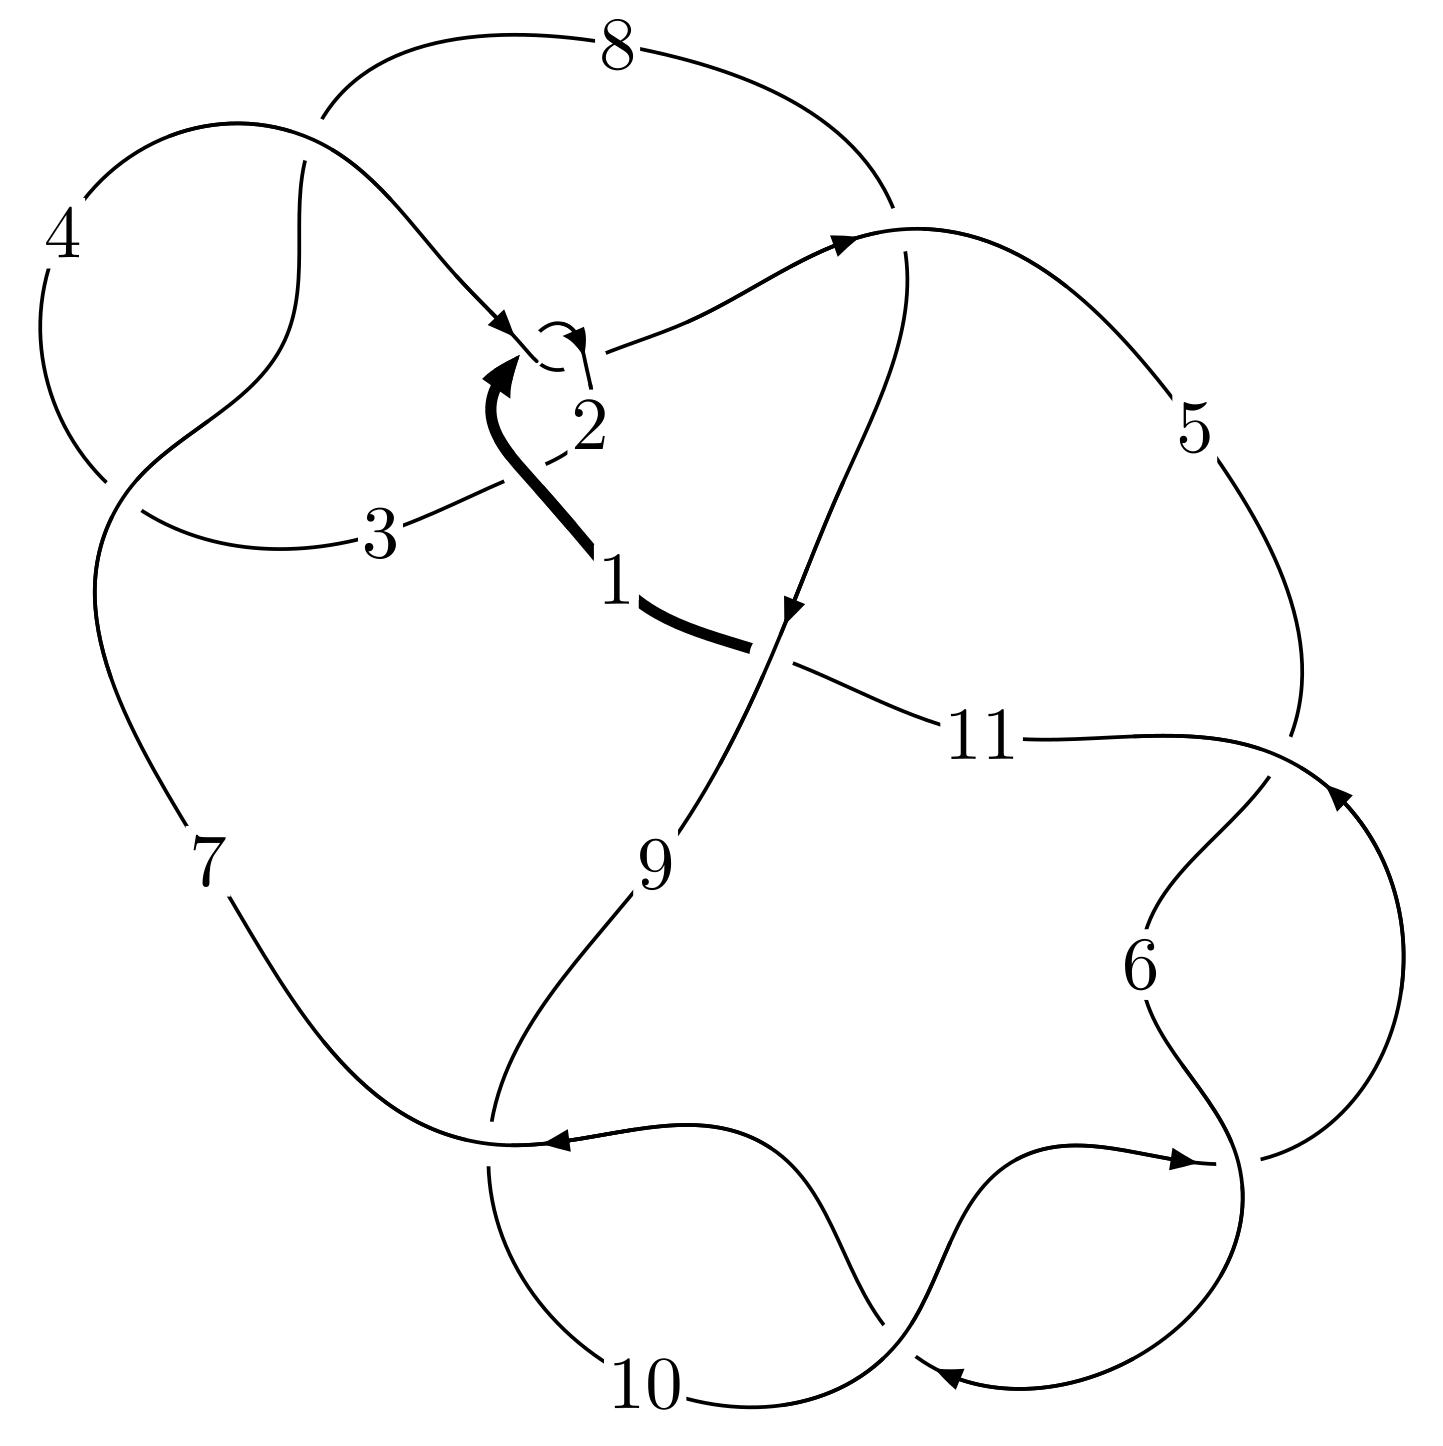
\includegraphics[width=112pt]{../../../GIT/diagram.site/Diagrams/png/679_11n_63.png}\\
\ \ \ A knot diagram\footnotemark}&
\allowdisplaybreaks
\textbf{Linearized knot diagam} \\
\cline{2-2}
 &
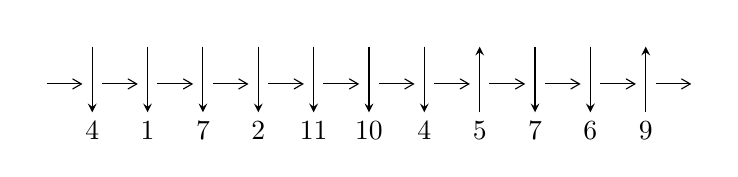
\begin{tikzpicture}[x=20pt, y=17pt]
	% nodes
	\node (C0) at (0, 0) {};
	\node (C1) at (1, 0) {};
	\node (C1U) at (1, +1) {};
	\node (C1D) at (1, -1) {4};

	\node (C2) at (2, 0) {};
	\node (C2U) at (2, +1) {};
	\node (C2D) at (2, -1) {1};

	\node (C3) at (3, 0) {};
	\node (C3U) at (3, +1) {};
	\node (C3D) at (3, -1) {7};

	\node (C4) at (4, 0) {};
	\node (C4U) at (4, +1) {};
	\node (C4D) at (4, -1) {2};

	\node (C5) at (5, 0) {};
	\node (C5U) at (5, +1) {};
	\node (C5D) at (5, -1) {11};

	\node (C6) at (6, 0) {};
	\node (C6U) at (6, +1) {};
	\node (C6D) at (6, -1) {10};

	\node (C7) at (7, 0) {};
	\node (C7U) at (7, +1) {};
	\node (C7D) at (7, -1) {4};

	\node (C8) at (8, 0) {};
	\node (C8U) at (8, +1) {};
	\node (C8D) at (8, -1) {5};

	\node (C9) at (9, 0) {};
	\node (C9U) at (9, +1) {};
	\node (C9D) at (9, -1) {7};

	\node (C10) at (10, 0) {};
	\node (C10U) at (10, +1) {};
	\node (C10D) at (10, -1) {6};

	\node (C11) at (11, 0) {};
	\node (C11U) at (11, +1) {};
	\node (C11D) at (11, -1) {9};
	\node (C12) at (12, 0) {};

	% arrows
	\draw[->,>={angle 60}]
	(C0) edge (C1) (C1) edge (C2) (C2) edge (C3) (C3) edge (C4) (C4) edge (C5) (C5) edge (C6) (C6) edge (C7) (C7) edge (C8) (C8) edge (C9) (C9) edge (C10) (C10) edge (C11) (C11) edge (C12) ;	\draw[->,>=stealth]
	(C1U) edge (C1D) (C2U) edge (C2D) (C3U) edge (C3D) (C4U) edge (C4D) (C5U) edge (C5D) (C6U) edge (C6D) (C7U) edge (C7D) (C8D) edge (C8U) (C9U) edge (C9D) (C10U) edge (C10D) (C11D) edge (C11U) ;
	\end{tikzpicture} \\
\hhline{~~} \\& 
\textbf{Solving Sequence} \\ \cline{2-2} 
 &
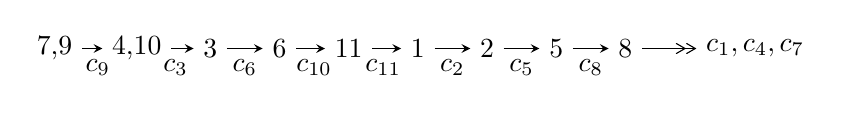
\begin{tikzpicture}[x=25pt, y=7pt]
	% node
	\node (A0) at (-1/8, 0) {7,9};
	\node (A1) at (17/16, 0) {4,10};
	\node (A2) at (17/8, 0) {3};
	\node (A3) at (25/8, 0) {6};
	\node (A4) at (33/8, 0) {11};
	\node (A5) at (41/8, 0) {1};
	\node (A6) at (49/8, 0) {2};
	\node (A7) at (57/8, 0) {5};
	\node (A8) at (65/8, 0) {8};
	\node (C1) at (1/2, -1) {$c_{9}$};
	\node (C2) at (13/8, -1) {$c_{3}$};
	\node (C3) at (21/8, -1) {$c_{6}$};
	\node (C4) at (29/8, -1) {$c_{10}$};
	\node (C5) at (37/8, -1) {$c_{11}$};
	\node (C6) at (45/8, -1) {$c_{2}$};
	\node (C7) at (53/8, -1) {$c_{5}$};
	\node (C8) at (61/8, -1) {$c_{8}$};
	\node (A9) at (10, 0) {$c_{1},c_{4},c_{7}$};

	% edge
	\draw[->,>=stealth]	
	(A0) edge (A1) (A1) edge (A2) (A2) edge (A3) (A3) edge (A4) (A4) edge (A5) (A5) edge (A6) (A6) edge (A7) (A7) edge (A8) ;
	\draw[->>,>={angle 60}]	
	(A8) edge (A9);
\end{tikzpicture} \\ 

\end{tabular} \\

\footnotetext{
The image of knot diagram is generated by the software ``\textbf{Draw programme}" developed by Andrew Bartholomew(\url{http://www.layer8.co.uk/maths/draw/index.htm\#Running-draw}), where we modified some parts for our purpose(\url{https://github.com/CATsTAILs/LinksPainter}).
}\phantom \\ \newline 
\centering \textbf{Ideals for irreducible components\footnotemark of $X_{\text{par}}$} 
 
\begin{align*}
I^u_{1}&=\langle 
- u^{14}-8 u^{12}-23 u^{10}-28 u^8-14 u^6+2 u^5-4 u^4+6 u^3+u^2+b+2 u,\;- u^{22}+u^{21}+\cdots+a-1,\\
\phantom{I^u_{1}}&\phantom{= \langle  }u^{23}-2 u^{22}+\cdots+12 u^3+1\rangle \\
I^u_{2}&=\langle 
- u^3- u^2+b-2 u-1,\;a,\;u^4+u^3+3 u^2+2 u+1\rangle \\
\\
\end{align*}
\raggedright * 2 irreducible components of $\dim_{\mathbb{C}}=0$, with total 27 representations.\\
\footnotetext{All coefficients of polynomials are rational numbers. But the coefficients are sometimes approximated in decimal forms when there is not enough margin.}
\newpage
\renewcommand{\arraystretch}{1}
\centering \section*{I. $I^u_{1}= \langle - u^{14}-8 u^{12}+\cdots+b+2 u,\;- u^{22}+u^{21}+\cdots+a-1,\;u^{23}-2 u^{22}+\cdots+12 u^3+1 \rangle$}
\flushleft \textbf{(i) Arc colorings}\\
\begin{tabular}{m{7pt} m{180pt} m{7pt} m{180pt} }
\flushright $a_{7}=$&$\begin{pmatrix}0\\u\end{pmatrix}$ \\
\flushright $a_{9}=$&$\begin{pmatrix}1\\0\end{pmatrix}$ \\
\flushright $a_{4}=$&$\begin{pmatrix}u^{22}- u^{21}+\cdots+4 u^2+1\\u^{14}+8 u^{12}+23 u^{10}+28 u^8+14 u^6-2 u^5+4 u^4-6 u^3- u^2-2 u\end{pmatrix}$ \\
\flushright $a_{10}=$&$\begin{pmatrix}1\\u^2\end{pmatrix}$ \\
\flushright $a_{3}=$&$\begin{pmatrix}u^{22}- u^{21}+\cdots+4 u^2+1\\u^{21}-2 u^{20}+\cdots- u+1\end{pmatrix}$ \\
\flushright $a_{6}=$&$\begin{pmatrix}u\\u^3+u\end{pmatrix}$ \\
\flushright $a_{11}=$&$\begin{pmatrix}u^2+1\\u^4+2 u^2\end{pmatrix}$ \\
\flushright $a_{1}=$&$\begin{pmatrix}u^4+3 u^2+1\\u^4+2 u^2\end{pmatrix}$ \\
\flushright $a_{2}=$&$\begin{pmatrix}- u^{13}-8 u^{11}-23 u^9-28 u^7-14 u^5+2 u^4-4 u^3+6 u^2+u+2\\- u^{22}+2 u^{21}+\cdots- u+1\end{pmatrix}$ \\
\flushright $a_{5}=$&$\begin{pmatrix}u^3+2 u\\u^5+3 u^3+u\end{pmatrix}$ \\
\flushright $a_{8}=$&$\begin{pmatrix}u^8+5 u^6+7 u^4+2 u^2+1\\u^{10}+6 u^8+11 u^6+6 u^4+u^2\end{pmatrix}$\\ \flushright $a_{8}=$&$\begin{pmatrix}u^8+5 u^6+7 u^4+2 u^2+1\\u^{10}+6 u^8+11 u^6+6 u^4+u^2\end{pmatrix}$\\&\end{tabular}
\flushleft \textbf{(ii) Obstruction class $= -1$}\\~\\
\flushleft \textbf{(iii) Cusp Shapes $= - u^{22}+2 u^{21}-16 u^{20}+27 u^{19}-108 u^{18}+155 u^{17}-403 u^{16}+495 u^{15}-916 u^{14}+969 u^{13}-1323 u^{12}+1215 u^{11}-1240 u^{10}+1001 u^9-769 u^8+558 u^7-333 u^6+218 u^5-114 u^4+53 u^3-24 u^2+3 u-5$}\\~\\
\newpage\renewcommand{\arraystretch}{1}
\flushleft \textbf{(iv) u-Polynomials at the component}\newline \\
\begin{tabular}{m{50pt}|m{274pt}}
Crossings & \hspace{64pt}u-Polynomials at each crossing \\
\hline $$\begin{aligned}c_{1},c_{4}\end{aligned}$$&$\begin{aligned}
&u^{23}-5 u^{22}+\cdots-4 u+1
\end{aligned}$\\
\hline $$\begin{aligned}c_{2}\end{aligned}$$&$\begin{aligned}
&u^{23}+5 u^{22}+\cdots+14 u+1
\end{aligned}$\\
\hline $$\begin{aligned}c_{3},c_{7}\end{aligned}$$&$\begin{aligned}
&u^{23}+u^{22}+\cdots+24 u+16
\end{aligned}$\\
\hline $$\begin{aligned}c_{5},c_{6},c_{9}\\c_{10}\end{aligned}$$&$\begin{aligned}
&u^{23}-2 u^{22}+\cdots+12 u^3+1
\end{aligned}$\\
\hline $$\begin{aligned}c_{8}\end{aligned}$$&$\begin{aligned}
&u^{23}-2 u^{22}+\cdots+2 u+1
\end{aligned}$\\
\hline $$\begin{aligned}c_{11}\end{aligned}$$&$\begin{aligned}
&u^{23}+8 u^{22}+\cdots+168 u+49
\end{aligned}$\\
\hline
\end{tabular}\\~\\
\newpage\renewcommand{\arraystretch}{1}
\flushleft \textbf{(v) Riley Polynomials at the component}\newline \\
\begin{tabular}{m{50pt}|m{274pt}}
Crossings & \hspace{64pt}Riley Polynomials at each crossing \\
\hline $$\begin{aligned}c_{1},c_{4}\end{aligned}$$&$\begin{aligned}
&y^{23}-5 y^{22}+\cdots+14 y-1
\end{aligned}$\\
\hline $$\begin{aligned}c_{2}\end{aligned}$$&$\begin{aligned}
&y^{23}+31 y^{22}+\cdots+14 y-1
\end{aligned}$\\
\hline $$\begin{aligned}c_{3},c_{7}\end{aligned}$$&$\begin{aligned}
&y^{23}+27 y^{22}+\cdots-2240 y-256
\end{aligned}$\\
\hline $$\begin{aligned}c_{5},c_{6},c_{9}\\c_{10}\end{aligned}$$&$\begin{aligned}
&y^{23}+28 y^{22}+\cdots+60 y^2-1
\end{aligned}$\\
\hline $$\begin{aligned}c_{8}\end{aligned}$$&$\begin{aligned}
&y^{23}-28 y^{22}+\cdots-40 y^2-1
\end{aligned}$\\
\hline $$\begin{aligned}c_{11}\end{aligned}$$&$\begin{aligned}
&y^{23}-16 y^{22}+\cdots+77224 y-2401
\end{aligned}$\\
\hline
\end{tabular}\\~\\
\newpage\flushleft \textbf{(vi) Complex Volumes and Cusp Shapes}
$$\begin{array}{c|c|c}  
\text{Solutions to }I^u_{1}& \I (\text{vol} + \sqrt{-1}CS) & \text{Cusp shape}\\
 \hline 
\begin{aligned}
u &= \phantom{-}0.430869 + 0.879813 I \\
a &= -1.53457 - 0.83314 I \\
b &= -0.032165 - 1.283100 I\end{aligned}
 & \phantom{-}7.83203 - 0.28979 I & -2.09012 + 1.34957 I \\ \hline\begin{aligned}
u &= \phantom{-}0.430869 - 0.879813 I \\
a &= -1.53457 + 0.83314 I \\
b &= -0.032165 + 1.283100 I\end{aligned}
 & \phantom{-}7.83203 + 0.28979 I & -2.09012 - 1.34957 I \\ \hline\begin{aligned}
u &= \phantom{-}0.506895 + 0.810130 I \\
a &= \phantom{-}1.71344 + 0.53833 I \\
b &= \phantom{-}0.75596 + 1.83026 I\end{aligned}
 & \phantom{-}7.20945 - 7.39071 I & -3.32519 + 6.20381 I \\ \hline\begin{aligned}
u &= \phantom{-}0.506895 - 0.810130 I \\
a &= \phantom{-}1.71344 - 0.53833 I \\
b &= \phantom{-}0.75596 - 1.83026 I\end{aligned}
 & \phantom{-}7.20945 + 7.39071 I & -3.32519 - 6.20381 I \\ \hline\begin{aligned}
u &= -0.257149 + 0.694856 I \\
a &= -0.700814 - 0.988990 I \\
b &= -0.828985 + 0.500798 I\end{aligned}
 & \phantom{-}0.92312 + 1.99790 I & -2.34638 - 5.92992 I \\ \hline\begin{aligned}
u &= -0.257149 - 0.694856 I \\
a &= -0.700814 + 0.988990 I \\
b &= -0.828985 - 0.500798 I\end{aligned}
 & \phantom{-}0.92312 - 1.99790 I & -2.34638 + 5.92992 I \\ \hline\begin{aligned}
u &= -0.474423 + 0.490062 I \\
a &= \phantom{-}0.599724 - 0.678621 I \\
b &= -0.223191 - 0.754283 I\end{aligned}
 & -0.68293 + 1.66090 I & -3.45266 - 4.83485 I \\ \hline\begin{aligned}
u &= -0.474423 - 0.490062 I \\
a &= \phantom{-}0.599724 + 0.678621 I \\
b &= -0.223191 + 0.754283 I\end{aligned}
 & -0.68293 - 1.66090 I & -3.45266 + 4.83485 I \\ \hline\begin{aligned}
u &= \phantom{-}0.679084 + 0.057677 I \\
a &= -0.18571 + 2.39295 I \\
b &= -0.49465 + 1.44023 I\end{aligned}
 & \phantom{-}4.95941 + 3.41645 I & -6.52166 - 2.22573 I \\ \hline\begin{aligned}
u &= \phantom{-}0.679084 - 0.057677 I \\
a &= -0.18571 - 2.39295 I \\
b &= -0.49465 - 1.44023 I\end{aligned}
 & \phantom{-}4.95941 - 3.41645 I & -6.52166 + 2.22573 I\\
 \hline 
 \end{array}$$\newpage$$\begin{array}{c|c|c}  
\text{Solutions to }I^u_{1}& \I (\text{vol} + \sqrt{-1}CS) & \text{Cusp shape}\\
 \hline 
\begin{aligned}
u &= \phantom{-}0.167283 + 0.490089 I \\
a &= \phantom{-}0.742425 + 0.936392 I \\
b &= \phantom{-}0.580042 - 0.782556 I\end{aligned}
 & -1.35992 - 0.76790 I & -3.34761 - 1.39618 I \\ \hline\begin{aligned}
u &= \phantom{-}0.167283 - 0.490089 I \\
a &= \phantom{-}0.742425 - 0.936392 I \\
b &= \phantom{-}0.580042 + 0.782556 I\end{aligned}
 & -1.35992 + 0.76790 I & -3.34761 + 1.39618 I \\ \hline\begin{aligned}
u &= -0.12264 + 1.52753 I \\
a &= -0.474160 + 0.043990 I \\
b &= \phantom{-}0.631841 + 0.749566 I\end{aligned}
 & \phantom{-}6.06133 + 3.74831 I & \phantom{-}0.03467 - 4.58469 I \\ \hline\begin{aligned}
u &= -0.12264 - 1.52753 I \\
a &= -0.474160 - 0.043990 I \\
b &= \phantom{-}0.631841 - 0.749566 I\end{aligned}
 & \phantom{-}6.06133 - 3.74831 I & \phantom{-}0.03467 + 4.58469 I \\ \hline\begin{aligned}
u &= \phantom{-}0.02397 + 1.58265 I \\
a &= -0.500609 - 0.414161 I \\
b &= -1.26560 + 1.17058 I\end{aligned}
 & \phantom{-}5.91283 - 1.29853 I & -3.45106 + 0.05233 I \\ \hline\begin{aligned}
u &= \phantom{-}0.02397 - 1.58265 I \\
a &= -0.500609 + 0.414161 I \\
b &= -1.26560 - 1.17058 I\end{aligned}
 & \phantom{-}5.91283 + 1.29853 I & -3.45106 - 0.05233 I \\ \hline\begin{aligned}
u &= -0.06369 + 1.61667 I \\
a &= \phantom{-}0.281195 + 0.690174 I \\
b &= \phantom{-}0.861442 - 0.947874 I\end{aligned}
 & \phantom{-}8.92549 + 3.15334 I & -1.05029 - 3.26062 I \\ \hline\begin{aligned}
u &= -0.06369 - 1.61667 I \\
a &= \phantom{-}0.281195 - 0.690174 I \\
b &= \phantom{-}0.861442 + 0.947874 I\end{aligned}
 & \phantom{-}8.92549 - 3.15334 I & -1.05029 + 3.26062 I \\ \hline\begin{aligned}
u &= \phantom{-}0.14770 + 1.64559 I \\
a &= -1.073510 + 0.242410 I \\
b &= -0.89607 - 2.20609 I\end{aligned}
 & \phantom{-}15.6090 - 9.9000 I & -1.58759 + 4.90312 I \\ \hline\begin{aligned}
u &= \phantom{-}0.14770 - 1.64559 I \\
a &= -1.073510 - 0.242410 I \\
b &= -0.89607 + 2.20609 I\end{aligned}
 & \phantom{-}15.6090 + 9.9000 I & -1.58759 - 4.90312 I\\
 \hline 
 \end{array}$$\newpage$$\begin{array}{c|c|c}  
\text{Solutions to }I^u_{1}& \I (\text{vol} + \sqrt{-1}CS) & \text{Cusp shape}\\
 \hline 
\begin{aligned}
u &= \phantom{-}0.11544 + 1.66378 I \\
a &= \phantom{-}1.121440 + 0.050156 I \\
b &= \phantom{-}0.53774 + 1.34352 I\end{aligned}
 & \phantom{-}16.6150 - 2.3845 I & -0.450202 + 0.532296 I \\ \hline\begin{aligned}
u &= \phantom{-}0.11544 - 1.66378 I \\
a &= \phantom{-}1.121440 - 0.050156 I \\
b &= \phantom{-}0.53774 - 1.34352 I\end{aligned}
 & \phantom{-}16.6150 + 2.3845 I & -0.450202 - 0.532296 I \\ \hline\begin{aligned}
u &= -0.306699\phantom{ +0.000000I} \\
a &= \phantom{-}2.02230\phantom{ +0.000000I} \\
b &= \phantom{-}0.747269\phantom{ +0.000000I}\end{aligned}
 & -0.900453\phantom{ +0.000000I} & -11.8240\phantom{ +0.000000I}\\
 \hline 
 \end{array}$$\newpage\newpage\renewcommand{\arraystretch}{1}
\centering \section*{II. $I^u_{2}= \langle - u^3- u^2+b-2 u-1,\;a,\;u^4+u^3+3 u^2+2 u+1 \rangle$}
\flushleft \textbf{(i) Arc colorings}\\
\begin{tabular}{m{7pt} m{180pt} m{7pt} m{180pt} }
\flushright $a_{7}=$&$\begin{pmatrix}0\\u\end{pmatrix}$ \\
\flushright $a_{9}=$&$\begin{pmatrix}1\\0\end{pmatrix}$ \\
\flushright $a_{4}=$&$\begin{pmatrix}0\\u^3+u^2+2 u+1\end{pmatrix}$ \\
\flushright $a_{10}=$&$\begin{pmatrix}1\\u^2\end{pmatrix}$ \\
\flushright $a_{3}=$&$\begin{pmatrix}0\\u^3+u^2+2 u+1\end{pmatrix}$ \\
\flushright $a_{6}=$&$\begin{pmatrix}u\\u^3+u\end{pmatrix}$ \\
\flushright $a_{11}=$&$\begin{pmatrix}u^2+1\\- u^3- u^2-2 u-1\end{pmatrix}$ \\
\flushright $a_{1}=$&$\begin{pmatrix}- u^3-2 u\\- u^3- u^2-2 u-1\end{pmatrix}$ \\
\flushright $a_{2}=$&$\begin{pmatrix}- u^3-2 u\\0\end{pmatrix}$ \\
\flushright $a_{5}=$&$\begin{pmatrix}u^3+2 u\\u^3+u^2+2 u+1\end{pmatrix}$ \\
\flushright $a_{8}=$&$\begin{pmatrix}0\\u\end{pmatrix}$\\ \flushright $a_{8}=$&$\begin{pmatrix}0\\u\end{pmatrix}$\\&\end{tabular}
\flushleft \textbf{(ii) Obstruction class $= 1$}\\~\\
\flushleft \textbf{(iii) Cusp Shapes $= -5 u^3-5 u^2-14 u-16$}\\~\\
\newpage\renewcommand{\arraystretch}{1}
\flushleft \textbf{(iv) u-Polynomials at the component}\newline \\
\begin{tabular}{m{50pt}|m{274pt}}
Crossings & \hspace{64pt}u-Polynomials at each crossing \\
\hline $$\begin{aligned}c_{1}\end{aligned}$$&$\begin{aligned}
&(u-1)^4
\end{aligned}$\\
\hline $$\begin{aligned}c_{2},c_{4}\end{aligned}$$&$\begin{aligned}
&(u+1)^4
\end{aligned}$\\
\hline $$\begin{aligned}c_{3},c_{7}\end{aligned}$$&$\begin{aligned}
&u^4
\end{aligned}$\\
\hline $$\begin{aligned}c_{5},c_{6}\end{aligned}$$&$\begin{aligned}
&u^4- u^3+3 u^2-2 u+1
\end{aligned}$\\
\hline $$\begin{aligned}c_{8},c_{11}\end{aligned}$$&$\begin{aligned}
&u^4+u^3+u^2+1
\end{aligned}$\\
\hline $$\begin{aligned}c_{9},c_{10}\end{aligned}$$&$\begin{aligned}
&u^4+u^3+3 u^2+2 u+1
\end{aligned}$\\
\hline
\end{tabular}\\~\\
\newpage\renewcommand{\arraystretch}{1}
\flushleft \textbf{(v) Riley Polynomials at the component}\newline \\
\begin{tabular}{m{50pt}|m{274pt}}
Crossings & \hspace{64pt}Riley Polynomials at each crossing \\
\hline $$\begin{aligned}c_{1},c_{2},c_{4}\end{aligned}$$&$\begin{aligned}
&(y-1)^4
\end{aligned}$\\
\hline $$\begin{aligned}c_{3},c_{7}\end{aligned}$$&$\begin{aligned}
&y^4
\end{aligned}$\\
\hline $$\begin{aligned}c_{5},c_{6},c_{9}\\c_{10}\end{aligned}$$&$\begin{aligned}
&y^4+5 y^3+7 y^2+2 y+1
\end{aligned}$\\
\hline $$\begin{aligned}c_{8},c_{11}\end{aligned}$$&$\begin{aligned}
&y^4+y^3+3 y^2+2 y+1
\end{aligned}$\\
\hline
\end{tabular}\\~\\
\newpage\flushleft \textbf{(vi) Complex Volumes and Cusp Shapes}
$$\begin{array}{c|c|c}  
\text{Solutions to }I^u_{2}& \I (\text{vol} + \sqrt{-1}CS) & \text{Cusp shape}\\
 \hline 
\begin{aligned}
u &= -0.395123 + 0.506844 I \\
a &= \phantom{-0.000000 } 0 \\
b &= \phantom{-}0.351808 + 0.720342 I\end{aligned}
 & -1.85594 + 1.41510 I & -11.17855 - 5.62908 I \\ \hline\begin{aligned}
u &= -0.395123 - 0.506844 I \\
a &= \phantom{-0.000000 } 0 \\
b &= \phantom{-}0.351808 - 0.720342 I\end{aligned}
 & -1.85594 - 1.41510 I & -11.17855 + 5.62908 I \\ \hline\begin{aligned}
u &= -0.10488 + 1.55249 I \\
a &= \phantom{-0.000000 } 0 \\
b &= -0.851808 - 0.911292 I\end{aligned}
 & \phantom{-}5.14581 + 3.16396 I & -6.32145 - 1.65351 I \\ \hline\begin{aligned}
u &= -0.10488 - 1.55249 I \\
a &= \phantom{-0.000000 } 0 \\
b &= -0.851808 + 0.911292 I\end{aligned}
 & \phantom{-}5.14581 - 3.16396 I & -6.32145 + 1.65351 I\\
 \hline 
 \end{array}$$\newpage
\newpage\renewcommand{\arraystretch}{1}
\centering \section*{ III. u-Polynomials}
\begin{tabular}{m{50pt}|m{274pt}}
Crossings & \hspace{64pt}u-Polynomials at each crossing \\
\hline $$\begin{aligned}c_{1}\end{aligned}$$&$\begin{aligned}
&((u-1)^4)(u^{23}-5 u^{22}+\cdots-4 u+1)
\end{aligned}$\\
\hline $$\begin{aligned}c_{2}\end{aligned}$$&$\begin{aligned}
&((u+1)^4)(u^{23}+5 u^{22}+\cdots+14 u+1)
\end{aligned}$\\
\hline $$\begin{aligned}c_{3},c_{7}\end{aligned}$$&$\begin{aligned}
&u^4(u^{23}+u^{22}+\cdots+24 u+16)
\end{aligned}$\\
\hline $$\begin{aligned}c_{4}\end{aligned}$$&$\begin{aligned}
&((u+1)^4)(u^{23}-5 u^{22}+\cdots-4 u+1)
\end{aligned}$\\
\hline $$\begin{aligned}c_{5},c_{6}\end{aligned}$$&$\begin{aligned}
&(u^4- u^3+3 u^2-2 u+1)(u^{23}-2 u^{22}+\cdots+12 u^3+1)
\end{aligned}$\\
\hline $$\begin{aligned}c_{8}\end{aligned}$$&$\begin{aligned}
&(u^4+u^3+u^2+1)(u^{23}-2 u^{22}+\cdots+2 u+1)
\end{aligned}$\\
\hline $$\begin{aligned}c_{9},c_{10}\end{aligned}$$&$\begin{aligned}
&(u^4+u^3+3 u^2+2 u+1)(u^{23}-2 u^{22}+\cdots+12 u^3+1)
\end{aligned}$\\
\hline $$\begin{aligned}c_{11}\end{aligned}$$&$\begin{aligned}
&(u^4+u^3+u^2+1)(u^{23}+8 u^{22}+\cdots+168 u+49)
\end{aligned}$\\
\hline
\end{tabular}\newpage\renewcommand{\arraystretch}{1}
\centering \section*{ IV. Riley Polynomials}
\begin{tabular}{m{50pt}|m{274pt}}
Crossings & \hspace{64pt}Riley Polynomials at each crossing \\
\hline $$\begin{aligned}c_{1},c_{4}\end{aligned}$$&$\begin{aligned}
&((y-1)^4)(y^{23}-5 y^{22}+\cdots+14 y-1)
\end{aligned}$\\
\hline $$\begin{aligned}c_{2}\end{aligned}$$&$\begin{aligned}
&((y-1)^4)(y^{23}+31 y^{22}+\cdots+14 y-1)
\end{aligned}$\\
\hline $$\begin{aligned}c_{3},c_{7}\end{aligned}$$&$\begin{aligned}
&y^4(y^{23}+27 y^{22}+\cdots-2240 y-256)
\end{aligned}$\\
\hline $$\begin{aligned}c_{5},c_{6},c_{9}\\c_{10}\end{aligned}$$&$\begin{aligned}
&(y^4+5 y^3+7 y^2+2 y+1)(y^{23}+28 y^{22}+\cdots+60 y^2-1)
\end{aligned}$\\
\hline $$\begin{aligned}c_{8}\end{aligned}$$&$\begin{aligned}
&(y^4+y^3+3 y^2+2 y+1)(y^{23}-28 y^{22}+\cdots-40 y^2-1)
\end{aligned}$\\
\hline $$\begin{aligned}c_{11}\end{aligned}$$&$\begin{aligned}
&(y^4+y^3+3 y^2+2 y+1)(y^{23}-16 y^{22}+\cdots+77224 y-2401)
\end{aligned}$\\
\hline
\end{tabular}
\vskip 2pc
\end{document}